\documentclass[11 pt]{beamer}
\let\Tiny=\tiny

\usepackage{mathtools}
\usepackage{amsfonts}
\usepackage{amsmath}
\usepackage{graphicx}
\usepackage{pgfpages}
\usepackage[]{xcolor}
\usepackage{tikz}


\newcommand{\meo}[1]{\texttt{#1}} % My Eyes Only: notes just for me
\newcommand{\bigo}{\mathcal{O}}
\newcommand{\extra}[1]{{\color{purple} {#1}}}

\usetheme{default}
\usecolortheme{beaver}
\usefonttheme{serif}


\beamertemplatenavigationsymbolsempty
\setbeameroption{show notes}


\newif\ifpresstime
	\presstimefalse
	% \presstimetrue

\mode<presentation>{
	\setbeameroption{hide notes}
}
\mode<handout>{
	\setbeameroption{show notes}
	\pgfpagesuselayout{2 on 1}[letterpaper, border shrink=5mm]

}


\ifpresstime
		\renewcommand{\meo}[1]{}
		\date{April 13, 2018}
		\setbeameroption{hide notes}
	\else
		\setbeameroption{show notes}
		% \setbeameroption{show only notes}
		\date{\today}
	\fi

\usetikzlibrary{arrows, automata, shapes}
\tikzset{
		initial text = {\scriptsize{\textsc{start}}},
		initial distance = 1 pt,
		every initial by arrow/.style={->},
		initial below,
		elliptic state/.style={draw,rounded rectangle},
		accepting/.style ={thick, double}
	}


\title{Kleene's Theorem}
\author{James McFeeters}
\institute {Beloit College}
\begin{document}

\frame{
	\titlepage
}

\begin{frame}
	\frametitle{Basic Definitions}
	\begin{itemize}
		\item Symbol
		\pause
		\item Alphabet ($\Sigma$)
		\pause
		\item String / word
		\begin{itemize}
			\pause
			\item The empty string ($\lambda$)
			\pause
			\item $|\lambda| = 0$
		\end{itemize}
		\pause
		\item Language
	\end{itemize}
\end{frame}


\begin{frame}
	\frametitle{Regular Operations}
	\begin{itemize}
		\item Union
		\item Concatenation
		\item Kleene Closure
	\end{itemize}
\end{frame}

\begin{frame}
	\frametitle{Concatenation}
	\begin{columns}[T]
		\column{0.3\textwidth}
			\begin{block}{Strings}
				\begin{flalign*}
					w_1 &= ab &\\
					w_2 &= bc &\\
					w_1 w_2 &= abbc &\\
				\end{flalign*}
			\end{block}
		\column{0.5\textwidth}
		\pause
			\begin{block}{Languages}
				\begin{flalign*}
					AB &= \{ ab \mid a \in A, \, b \in B \} &\\
				\end{flalign*}
			\end{block}
	\end{columns}
	\begin{columns}[T]
		\column{0.3\textwidth}
		\pause
			\begin{flalign*}
				w^0 &= \lambda 		& \\
				w^1 &= w 			& \\
				w^2 &= ww			& \\
				w^k &= w w^{k-1} 	&
			\end{flalign*}
		\column{0.5\textwidth}
		\pause
			\begin{flalign*}
				A^0 &= \{ \lambda\} 					& \\
				A^1 &= A \{ \lambda \} = A 				& \\
				A^2 &= AA = \{ xy \mid x, y \in A \}	& \\
				A^k &= A A^{k-1}
			\end{flalign*}
	\end{columns}
\end{frame}

\begin{frame}
	\frametitle{Kleene Closure}
	$A^*$: the \textbf{Kleene closure} of $A$.
	\pause
	\begin{align*}
		A^* &= \bigcup_{k \geq 0} A^k \\
		&= \{ \lambda \} \cup A \cup A^2 \cdots \\
	\end{align*}
	\pause
	If $A = \{ y \}$ then $A^* = \{ \lambda, \: y, \: yy, \: yyy, \: \dots\}$.
\end{frame}

\begin{frame}
	\frametitle{Regular Languages}

	The \textbf{atomic} regular languages over an alphabet $\Sigma$ are
	\begin{itemize}
		\pause
		\item $\emptyset$
		\pause
		\item $\{ \lambda \}$
		\pause
		\item $\{ a \}$ for any $a \in \Sigma$ 
	\end{itemize}~\\[1 em]
	\pause

	If $A$ and $B$ are regular languages, then so are
	\begin{itemize}
		\pause
		\item $A \cup B$
		\pause
		\item $AB$
		\pause
		\item $A^*$
	\end{itemize}
\end{frame}

\begin{frame}
	\frametitle{Finite Automata}

	5-tuple: $M = (Q, \Sigma, s, \delta, F)$

	\begin{itemize}
		\pause
		\item [$Q$] The set of possible states.
		\pause
		\item [$\Sigma$] The alphabet of input symbols.
		\pause
		\item [$s$] The initial state, $s \in Q$.
		\pause
		\item [$\delta$] The transition function:
		\pause
		\[
			\delta: (Q \times \Sigma) \to Q.
		\]
		\pause
		\item [$F$] The set of accepting states, $F \subseteq Q$.
	\end{itemize}
\end{frame}




\begin{frame}
	\frametitle{Building a Finite Automaton}
	\begin{center}
	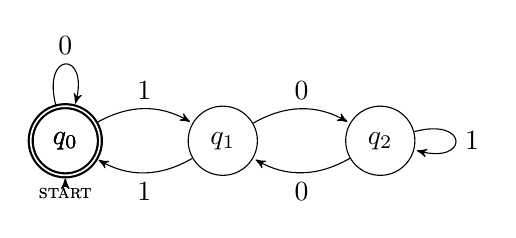
\begin{tikzpicture}[>=stealth',shorten >=1pt,auto,node distance=2cm]
		\pause % 1
		\temporal<3>
		{\node[state] (q0)                     {$q_0$};}
		{\node[state, initial] (q0)            {$q_0$};}
		{\node[state, initial, accepting] (q0) {$q_0$};}
		\node[state]                   (q1) [right of = q0] {$q_1$};
		\node[state]                   (q2) [right of = q1] {$q_2$};
		\pause % 2 Plain q0
		\pause % 3 Initial q0
		\pause % 4 Accepting q0
		\pause % 5 Show Sigma
		\path[->] (q0) edge [loop above] node {0} (q0);
		\pause % 6
		\path[->] (q0) edge [bend left]  node {1} (q1);
		\pause % 7
		\path[->] (q1) edge [bend left]  node {0} (q2);
		\pause % 8
		\path[->] (q1) edge [bend left]  node {1} (q0);
		\pause % 9
		\path[->] (q2) edge [bend left]  node {0} (q1);
		\pause % 10
		\path[->] (q2) edge [loop right] node {1} (q2);
	\end{tikzpicture}
	\end{center}
	\visible<2->{$Q = \{ q_0, q_1, q_2 \}$}\\
	\visible<3->{$s = q_0$}\\
	\visible<4->{$F = \{ q_0 \}$}\\
	\visible<5->{$\Sigma = \{ 0, 1 \}$}
	
\end{frame}

\note[itemize]{
	\item 
}

\begin{frame}
	\frametitle{More Fun with Automata}
	Extending the transition function:
	\pause
	\[
		\Delta : (Q \times \Sigma^*) \to Q
	\]
	\pause
	For $wa \in \Sigma^*$:
	\[
		\Delta(q_1, wa) = \delta(\Delta(q_1, w), a)
	\]
	\pause
	No transitions on $\lambda$:
	\[
		\delta(q_i, \lambda) = q_i
	\]
	\pause

	The machine \textbf{accepts} $w$ if $\Delta(s, w) \in F$.\\[2 ex]
	\pause

	A machine \textbf{represents} $A$ if $\Delta(s, w) \in F$ for all $w \in A$.
\end{frame}
\note[itemize]{
	\item We want to talk about the state of the machine after a string of inputs, not just after each symbol, so we want to extend the transition function
	\item So now we have a transition on any string, not just on a symbol.
	\item We don't transition on the empty string (although it's equally valid to define automata that have lambda-transitions.)
}

\begin{frame}
	\frametitle{Nondeterministic Automata}
	An automaton with multiple (or no) transitions from a state on a symbol?
	\pause

	\begin{center}
	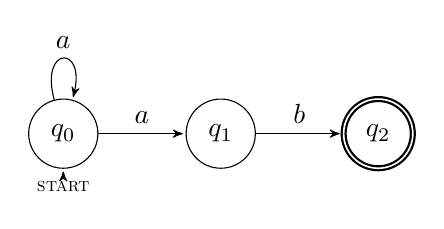
\begin{tikzpicture}[>=stealth',shorten >=1pt,auto,node distance=2cm]
		\node[state, initial]   (q0)                 {$q_0$};
		\node[state]            (q1) [right of = q0] {$q_1$};
		\node[state, accepting] (q2) [right of = q1] {$q_2$};

		\path[->] (q0) edge [loop above] node {$a$} (q0);
		\path[->] (q0) edge              node {$a$} (q1);
		\path[->] (q1) edge              node {$b$} (q2);
	\end{tikzpicture}
	\end{center}
	\pause
	Accepts $ab, \, aab, \, aaab, \dots$.
\end{frame}
\note[itemize]{
	\item All the automata we've dealt with so far have exactly one transition from each state on each input, but this is not actually required.
	\item We can build automata without this restriction: they are called nondeterministic, abbreviated to NDFA.
	\item This automaton has two transitions from $q_0$ on $a$, to itself and to $q_1$. 
			There is no transition from $q_1$ on $a$, and no transition from $q_0$ on $b$.
}

\begin{frame}
	\frametitle{NDFAs are Tricky}

\end{frame}

\begin{frame}
	\frametitle{Kleene's Theorem}
	A language is representable if and only if it is regular.
\end{frame}




\begin{frame}[shrink]
	\frametitle{References}
	\bibliographystyle{amsplain}
	\nocite{*}
	\bibliography{../paper/references.bib}
\end{frame}

\end{document}
